\documentclass{article} % For LaTeX2e
\usepackage{nips11submit_e,times}
\usepackage{graphicx}
%\documentstyle[nips10submit_09,times,art10]{article} % For LaTeX 2.09


\title{Perceptual Multistability in a Temporal Illusion}


\author{
Joseph Marrama \\
Department of Symbolic Systems\\
Stanford University\\
\texttt{jmarrama@stanford.edu} \\
\And
Alden Timme \\
Department of Math and Computational Sciences \\
Stanford University \\
\texttt{aotimme@stanford.edu} \\
}

% The \author macro works with any number of authors. There are two commands
% used to separate the names and addresses of multiple authors: \And and \AND.
%
% Using \And between authors leaves it to \LaTeX{} to determine where to break
% the lines. Using \AND forces a linebreak at that point. So, if \LaTeX{}
% puts 3 of 4 authors names on the first line, and the last on the second
% line, try using \AND instead of \And before the third author name.

\newcommand{\fix}{\marginpar{FIX}}
\newcommand{\new}{\marginpar{NEW}}

\nipsfinalcopy % Uncomment for camera-ready version

\begin{document}


\maketitle

\begin{abstract}
In this project, we model the cognitive conception of a visual illusion that can be perceived in four primary modes. 
We model perceptual multistability using a generative Bayesian network that captures the relations between high level features that are extracted from the illusion and the different overall conceptions of the illusion that the viewer can have.
Due to the high complexity of the illusion itself, we simplify the visual stimulus down to a single unit that corresponds to the viewer's observation of the visual stimulus.
Despite this simplifying assumption, our model is sophisticated enough to allow it to exhibit human-like perceptual multistability using Markov Chain Monte Carlo (MCMC) methods to sample from the model conditioned on the observed stimulus. (once we actually get results we should write the rest) 


%In this project, we model the cognitive conception of the reception of a visual field. Our model is a generative Bayesian one in which our uppermost variable represents the viewer’s conception of the visual field – i.e. the background structure of what the viewer sees. Rather than seeing the visual field as a sum of components, the model attempts to express the cognitive phenomenon of interpreting a visual stimulus as a whole cognitive concept. In an illusion, for example, we see one set of components which comprise the entire visual field, but this same set of components can yield multiple interpretations. Viewing this interpretive practice as a Bayesian model, we place the interpretation of the scene at the first layer in the hierarchy. This interpretation then provides a probability distribution over the variables at the second layer, which correspond to the perceived characteristics of the observed components that make up the visual stimulus. Finally, the set of all possible visual stimuli make up the third and final layer.
\end{abstract}


%so , how about an outline to start things off?
%i guess we should sorta shape the writeup like a paper, except much more specific on the model and 
%much shorter on the intro BS

%1. a short intro to perceptual multistability? introduce our illusion, etc....

%2. OUR MODEL - the basic structure, simplifying assumptions
%  question - include only the good gamma-distributed model or both??? which is 'more biologically plausable'?

%3. our results..... which mostly consist of switching times..... 
%  ALSO, model setting the clues in the illusion by setting certain illusion-type things to be constant...



\section{Perceptual Multistability}
%What should be our first section? We should probably do the model first..... 
The mental phenomenon of perceptual multistability is a commonly modeled aspect of human cognition, because it is a well-defined and well-measured phenomenon, and it is fairly easy to model simple illusions that give rise to multistability.
However, little research has gone into modeling perceptual multistability in complex illusions, such as those with a temporal component, multiple stable percepts, and complex structure. 
In our project, we aim to model a high-dimensional temporal illusion with 6 stable percepts (which can be found at bit.ly/c3uGK2) and accurately reconstruct the dynamics of perceptual multistability as it naturally arises from the illusion using MCMC sampling. 


\section{Our Model}
%simplifying the illusion itself, our model, simplifying the featureset, then simplifying the illusion 
Due to the high complexity of the illusion, a number of simplifying assumptions have to be made in order to construct a computationally tractable model. Before we constructed our model, we decided to reduce the number of stable percepts in the illusion to 4 instead of 6, because the mirror images of the double helix and wave forms (see the illusion) are very similar, to the point where they are practically interchangable. The difference between the helix, wave, horizontal motion, and bouncing dots percepts is much more significant than the difference between the 2 wave and helix configurations. 

Using this simplification, we constructed a 3-layer generative Bayesian network for our model. Each unit in each layer (except the bottom layer) contains directed edges going from that unit to every unit in the layer immediately below it. (figure would be nice) The top layer contains (4? a variable number?) 'percept' units, where each unit can take on a value 1 to 4 that corresponds to a different percept of the illusion. The top layer generates the second layer, which contains intermediate 'high-level feature' units that correspond to different characteristics one might observe. We have five of these units, which correspond to observed dimensionality (2d or 3d), planar rotation, horizontal velocity, correlation between dots in each column, and number of objects in the illusion. Lastly, the bottom layer captures the observed illusion. For the bottom layer, we model the input of the illusion as a single 'illusion unit', which has two values corresponding to whether the illusion is being observed or not. This is a very large but necessary simplification, because modeling configurations of the dots in the illusion would've taken hundreds of variables and a temporal model. Also, our approach is still wholly valid, because we can encode the configurations of high-level features that are likely to be observed in the illusion in the conditional probability distribution of the bottom-layer unit. For example, if a configuration of high-level features are observed that \emph{don't} correspond to any percept of the illusion (say, rotation and 2-dimensionality were observed), the illusion unit has a near-zero probability of being active, whereas if a configuration of high-level features that correspond to one of the percepts is observed, then the illusion unit has a near-one probability of being active.

%possibly add a section on more justification for our model? - woooorddddd
Our model can be viewed as a cognitive representation of the reception of a visual field. Staying true to the concepts taught in class, our model is a generative model, where each higher level of abstraction generates the lower. The model can be viewed as a small subset of the complete visual system, where we only use levels of abstraction and units that are relevant for modeling the illusion. To model the stimulus of the illusion, we condense all lower layers of abstraction/visual processing into a single layer of abstraction that represents all possible visual stimuli, and then only include the one unit that represents the stimuli of the illusion. 

The CPDs of all the variables in the model can be parameterized as follows. Let the second-layer 'high-level feature' units be denoted as $\{D, R, HV, CC, NO\}$, where they are in the same order as their enumeration above. Let the top-level percept units be denoted as $T_1, T_2, T_3, T_4$, the bottom-layer illusion unit as $I$, and finally, let the number of values a unit $U$ can take on be denoted as $|U|$.  

In the illusion, each stable percept corresponds to a unique assignment to the high-level feature units. Let $c_1$ denote this configuration for viewing the illusion as ovals moving horizontally, $c_2$ the configuration for the double helix, $c_3$ for the wave, and $c_4$ for the dots moving up and down. These are defined as:

\begin{eqnarray*}
c_1 &=& \{D_0,R_0,HV_1,CC_1,NO_1 \} \\
c_2 &=& \{D_1,R_1,HV_0,CC_1,NO_0 \} \\
c_3 &=& \{D_1,R_0,HV_0,CC_1,NO_0 \} \\
c_4 &=& \{D_0,R_0,HV_0,CC_0,NO_2 \} 
\end{eqnarray*}

The probability distributions for all top level units $T_i$ taking on different percepts is simply distributed according to a multinomial distribution whose parameters are given by a dirichlet distribution with hyper-parameters $\alpha = 200$ (in order to make it give a multinomial distribution close to the uniform distribution) and with a dimension of 4 (because there are 4 possible percepts).
%:
%\begin{eqnarray*}
%P(T_i = j) &=& 0.25 \\
%\end{eqnarray*}

In order to describe the probability distributions for all mid-layer units $ML$, lets define the following function:
\begin{eqnarray*}
\phi(T_i, ML_x) &=& (1-(|ML|-1)*\epsilon) \textrm{  if } T_i = j \textrm{ and } ML_x \in c_j \\
&=& (\epsilon) \textrm{  if } T_i = j \textrm{ and } ML_x \notin c_j \\
\end{eqnarray*}

Now, we can define:

\begin{eqnarray*}
P(ML = x|T_1,T_2,T_3,T_4) &=& \frac{\sum_{i=1}^4 \phi(T_i, ML_x)}{4} \\
\end{eqnarray*}

In more understandable terms, the probability $P(ML_x|T_1...T_4)$ is simply the average of all of the contributions of $T_1...T_4$, where the contribution of $T_i$ is simply $(1-\epsilon)$ if $ML_x$ corresponds to the assigned percept of $T_i$, or $\epsilon$ if not. $\epsilon$ can be viewed as a noise term.

Lastly, the CPD for the bottom unit $I$ is:
\begin{eqnarray*}
P(I=1|D,R,HV,CC,NO) &=& (1-\epsilon) \textrm{   if } c_i = \{D,R,HV,CC,NO\} \\
&=& \epsilon \textrm{   if } c_i \neq \{D,R,HV,CC,NO\}  
\end{eqnarray*}


\section{Results}
%how we parameterized the CPDs for the intermediate layer
For all experiments, we used standard Gibbs sampling as our MCMC sampling method, and sampled in order to approximate the posterior $P(M_{-I}|I_1)$, where $I_1$ means the illusion is on and $M_{-I}$ is the whole model sans $I$. Unless otherwise stated, we first sample all variables using forward sampling (and set $I=1$), then use a burn-in time of 10,000 Gibbs samples, and then collect 1,000,000 samples. 
For the experiments discussed below, we use a noise parameter of $\epsilon = 0.01$ and 4 top-level units $T_i$ unless otherwise stated. \\ 

%FUCK FUCK FUCK stupid fucking shit is hella hard to justify - FMLLLLLLLLL
%As a sanity check to make sure our model is working, we can use the resulting 1,000,000 samples to quickly calculate $P(T_i = j|I = 1)$.


\subsection{Distribution of dominance durations}
As you can see in the figure below, the time to switch between dominant percepts is roughly distributed according to a gamma distribution. We define a 'dominant percept' as anytime 3 or more top-layer percept units are assigned the same percept. It has been thoroughly documented that switching times in humans between different stable percepts tend to follow a Gamma distribution. Our model has similar behavior. This is likely because each top-layer percept unit has switching times roughly distributed along an exponential distribution, and the Gamma distribution is just a sum of exponential distributions. Nonetheless, our model exhibits human-like characteristics, which is a success of our model. \\

%(insert image and small text beneath it...)
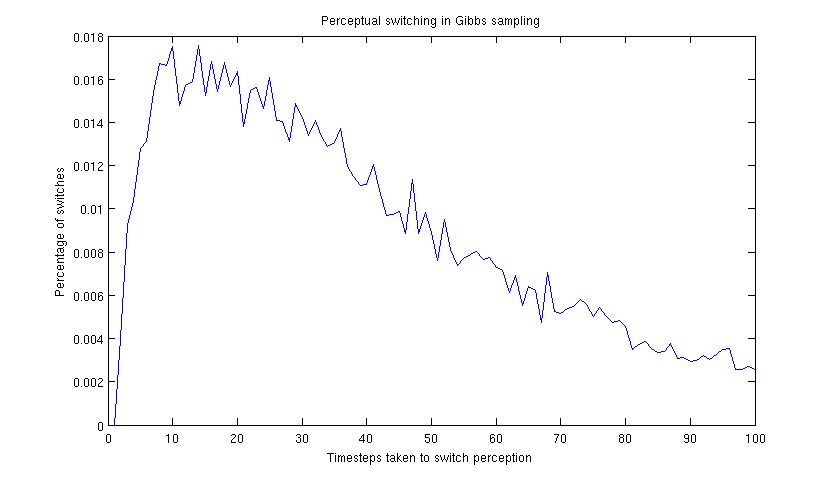
\includegraphics[scale=0.51]{1milUniformPfinal}
\small{herro}


\subsection{Visual Cues}
In the illusion, there are certain visual cues you can set that help you see different percepts. For example, the horizontal motion cue displays a dot moving along with each object to cue the viewer into the fact that there are multiple objects moving along at a high horizontal velocity. This provides a unique opportunity to test our model by holding these cues constant and sampling from the new posterior $P(M_{-I-cues}|I=1, cues)$, and then using the resulting samples to approximate $P(T_i|I=1, cues)$. Intuitively, we should expect $P(T_i = j|I=1, cues)$ ,assuming the cues are for percept $j$


\section{Discussion}

















\newpage

COOL \LaTeXe STUFF!!! alright! LOL?

\subsection{Footnotes}

Indicate footnotes with a number\footnote{Sample of the first footnote} in the
text. Place the footnotes at the bottom of the page on which they appear.
Precede the footnote with a horizontal rule of 2~inches
(12~picas).\footnote{Sample of the second footnote}

\subsection{Figures}

All artwork must be neat, clean, and legible. Lines should be dark
enough for purposes of reproduction; art work should not be
hand-drawn. The figure number and caption always appear after the
figure. Place one line space before the figure caption, and one line
space after the figure. The figure caption is lower case (except for
first word and proper nouns); figures are numbered consecutively.

Make sure the figure caption does not get separated from the figure.
Leave sufficient space to avoid splitting the figure and figure caption.

You may use color figures. 
However, it is best for the
figure captions and the paper body to make sense if the paper is printed
either in black/white or in color.
\begin{figure}[h]
\begin{center}
%\framebox[4.0in]{$\;$}
\fbox{\rule[-.5cm]{0cm}{4cm} \rule[-.5cm]{4cm}{0cm}}
\end{center}
\caption{Sample figure caption.}
\end{figure}

\subsection{Tables}

All tables must be centered, neat, clean and legible. Do not use hand-drawn
tables. The table number and title always appear before the table. See
Table~\ref{sample-table}.

Place one line space before the table title, one line space after the table
title, and one line space after the table. The table title must be lower case
(except for first word and proper nouns); tables are numbered consecutively.

\begin{table}[t]
\caption{Sample table title}
\label{sample-table}
\begin{center}
\begin{tabular}{ll}
\multicolumn{1}{c}{\bf PART}  &\multicolumn{1}{c}{\bf DESCRIPTION}
\\ \hline \\
Dendrite         &Input terminal \\
Axon             &Output terminal \\
Soma             &Cell body (contains cell nucleus) \\
\end{tabular}
\end{center}
\end{table}

LaTeX users:

\begin{itemize}

\item Consider directly generating PDF files using \verb+pdflatex+
(especially if you are a MiKTeX user). 
PDF figures must be substituted for EPS figures, however.

\item Otherwise, please generate your PostScript and PDF files with the following commands:
\begin{verbatim} 
dvips mypaper.dvi -t letter -Ppdf -G0 -o mypaper.ps
ps2pdf mypaper.ps mypaper.pdf
\end{verbatim}

Check that the PDF files only contains Type 1 fonts. 
%For the final version, please send us both the Postscript file and
%the PDF file. 

\item xfig "patterned" shapes are implemented with 
bitmap fonts.  Use "solid" shapes instead. 
\item The \verb+\bbold+ package almost always uses bitmap
fonts.  You can try the equivalent AMS Fonts with command
\begin{verbatim}
\usepackage[psamsfonts]{amssymb}
\end{verbatim}
 or use the following workaround for reals, natural and complex: 
\begin{verbatim}
\newcommand{\RR}{I\!\!R} %real numbers
\newcommand{\Nat}{I\!\!N} %natural numbers 
\newcommand{\CC}{I\!\!\!\!C} %complex numbers
\end{verbatim}

\item Sometimes the problematic fonts are used in figures
included in LaTeX files. The ghostscript program \verb+eps2eps+ is the simplest
way to clean such figures. For black and white figures, slightly better
results can be achieved with program \verb+potrace+.
\end{itemize}

\subsubsection*{Acknowledgments}

Use unnumbered third level headings for the acknowledgments. All
acknowledgments go at the end of the paper. Do not include 
acknowledgments in the anonymized submission, only in the 
final paper. 

\subsubsection*{References}

References follow the acknowledgments. Use unnumbered third level heading for
the references. Any choice of citation style is acceptable as long as you are
consistent. It is permissible to reduce the font size to `small' (9-point) 
when listing the references. {\bf Remember that this year you can use
a ninth page as long as it contains \emph{only} cited references.}

\small{
[1] Alexander, J.A. \& Mozer, M.C. (1995) Template-based algorithms
for connectionist rule extraction. In G. Tesauro, D. S. Touretzky
and T.K. Leen (eds.), {\it Advances in Neural Information Processing
Systems 7}, pp. 609-616. Cambridge, MA: MIT Press.

[2] Bower, J.M. \& Beeman, D. (1995) {\it The Book of GENESIS: Exploring
Realistic Neural Models with the GEneral NEural SImulation System.}
New York: TELOS/Springer-Verlag.

[3] Hasselmo, M.E., Schnell, E. \& Barkai, E. (1995) Dynamics of learning
and recall at excitatory recurrent synapses and cholinergic modulation
in rat hippocampal region CA3. {\it Journal of Neuroscience}
{\bf 15}(7):5249-5262.
}

\end{document}
